\documentclass[onecolumn, draftclsnofoot,10pt, compsoc]{IEEEtran}
\usepackage{graphicx}
\usepackage{url}
\usepackage{setspace}
\usepackage{pstricks-add}
\usepackage{float}
\usepackage{soul}
\usepackage{color}

\usepackage{listings}


% COLOR DEFINITIONS FOR CODE LISTINGS
\definecolor{codegreen}{rgb}{0,0.6,0}
\definecolor{codegray}{rgb}{0.5,0.5,0.5}
\definecolor{codepurple}{rgb}{0.58,0,0.82}
\definecolor{backcolour}{rgb}{0.95,0.95,0.92}

\lstdefinestyle{mystyle}{
    backgroundcolor=\color{backcolour},
    commentstyle=\color{codegreen},
    keywordstyle=\color{magenta},
    numberstyle=\tiny\color{codegray},
    stringstyle=\color{codepurple},
    basicstyle=\footnotesize,
    breakatwhitespace=false,
    breaklines=true,
    captionpos=b,
    keepspaces=true,
    numbers=left,
    numbersep=5pt,
    showspaces=false,
    showstringspaces=false,
    showtabs=false,
    tabsize=2
}

\lstset{
	escapeinside={(*@}{@*)},
	style=mystyle
}

\usepackage{geometry}
\geometry{textheight=9.5in, textwidth=7in}

% 1. Fill in these details
\def \CapstoneTeamName{		AKA Robotics}
\def \CapstoneTeamNumber{		13}
\def \GroupMemberOne{     Arthur Shing}
\def \GroupMemberTwo{	Kevin Talik}
\def \GroupMemberThree{   Anish Asrani}
\def \CapstoneProjectName{		How to Make an Effective Robot Comedian}
\def \CapstoneSponsorCompany{	Oregon State University}
\def \CapstoneSponsorPerson{		Heather Knight}

% 2. Uncomment the appropriate line below so that the document type works
\def \DocType{		%Problem Statement
				%Requirements Document
				%Technology Review
				%Design Document
				Progress Report
				}

\newcommand{\NameSigPair}[1]{\par
\makebox[2.75in][r]{#1} \hfil 	\makebox[3.25in]{\makebox[2.25in]{\hrulefill} \hfill		\makebox[.75in]{\hrulefill}}
\par\vspace{-12pt} \textit{\tiny\noindent
\makebox[2.75in]{} \hfil		\makebox[3.25in]{\makebox[2.25in][r]{Signature} \hfill	\makebox[.75in][r]{Date}}}}
% 3. If the document is not to be signed, uncomment the RENEWcommand below
\renewcommand{\NameSigPair}[1]{#1}

%%%%%%%%%%%%%%%%%%%%%%%%%%%%%%%%%%%%%%%
\begin{document}

\bstctlcite{IEEEexample:BSTcontrol}
\begin{titlepage}
    \pagenumbering{gobble}
    \begin{singlespace}
        \hfill
        % 4. If you have a logo, use this includegraphics command to put it on the coversheet.
        %\includegraphics[height=4cm]{CompanyLogo}
        \par\vspace{.2in}
        \centering
        \scshape{
            \huge CS Capstone \DocType \par
            {\large\today}\par
            \vspace{.5in}
            \textbf{\Huge\CapstoneProjectName}\par
            \vfill
            {\large Prepared for}\par
            \Huge \CapstoneSponsorCompany\par
            \vspace{5pt}
            {\Large\NameSigPair{\CapstoneSponsorPerson}\par}
            {\large Prepared by }\par
            Group\CapstoneTeamNumber\par
            % 5. comment out the line below this one if you do not wish to name your team
            \CapstoneTeamName\par
            \vspace{5pt}
            {\Large
                \NameSigPair{\GroupMemberOne}\par
                \NameSigPair{\GroupMemberTwo}\par
                \NameSigPair{\GroupMemberThree}\par
            }
            \vspace{20pt}
        }
        \begin{abstract}
Human-Robot interaction can learn a lot from stand-up comedy. A stand-up set has scripted jokes, statements that are predetermined,
as well as improvisational statements, that give the performance a sense of liveliness and character. A comedian can observe
an audience and improvise a delivery of a joke to connect the audience to the content. This makes the experience more authentic and
genuine for the observer. The purpose of this project is to to discover what makes an entertaining interaction by studying a robot that
performs comedy. We propose that a performance is enhanced when (1) the comedian interacts spontaneously with the audience,
(2) the comedian has and conveys a coherent, well-developed character, and (3) the comedian adapts its act to cater to an audience
based on their reaction. These propositions will be tested locally, remotely, and in a real stand-up setting.
	\end{abstract}
    \end{singlespace}
\end{titlepage}
\newpage
\pagenumbering{arabic}
\tableofcontents
% 7. uncomment this (if applicable). Consider adding a page break.
%\listoffigures
%\listoftables
\clearpage

% 8. now you write!
\section{Recap}

A lot of the machines that surround us aren't very engaging to interact with. They serve their purpose, people get what they need, and the interaction is over. People do not consider robots as entities. That is the gap we are trying to close by performing stand-up comedy with a robot. Stand-up comedy is a casual and entertaining way for people to get more exposure to robots and see that robots are not just objects, but they are much more than that.

An effective robot comedian should be able to entertain the audience and generate laughs. We hypothesize that the effectiveness is dependent on three major aspects - crowd-work or the ability to integrate the audience in the performance, portraying a coherent and convincing character, and the ability to adapt the performance based on audience feedback. We will base our performances and studies around these three areas.


\section{Kevin Talik}
    This section of the report will cover the adaptation algorithm in the scope of this project. First, there will be a review of the goals in studying adaptation during a performance. The next section will summarize the current progress that has been made in implementing adaptive transitions. Concluding this subsection of this group report will be a list of what next steps need to be taken, and current problems that are impeding the progress.   

     At a high level, the adaptation algorithm in this project will structure individual jokes into one performance set. The two goals of this result are: (1) to transition to topics dependent on the
  audience response, and (2) to present a crowd report upon completion of the set. The reason for presenting a crowd report back to the audience after the performance is that people may not notice actions the robot is taking to connect to the crowd. 
\subsection{Progress So Far}
    This term has been focusing on putting our individual work into one, cohesive program that will run. The adaptation algorithm needs multiple jokes during the same performing cycle to compare what the audience like.  We have animated eight jokes total, and have five that are currently in a single performance. Each joke that is physically animated in the robot will need a Python Object that describes the heuristics of the joke. Each joke object is appended to a list, and removed as they are performed. After the joke is told, the joke object will be pushed to a queue. The purpose of the queue is for the crowd report; each joke object will be popped off as they were told to construct the report of the audience. 


 Below, is a code snippit of initializing and arranging an example performance. This is helpful in testing, because verifying the animations needs to happen manually. Before implementing the crowd report, each animation needs to be safe for the robot; our comedian needs to be able to survive each set. This requires careful iterations of movements to make sure that it does not fall over.

    
    
\subsection{Left To Do}

\subsubsection{Methods}
Generally, the performance will have two to three parts: the Seed Jokes, the Middle Content, and the Close. The Seed will influence the Middle Content (which will be chosen themed jokes and basis of the show). The Middle Content will transition to a intelligent or generalized Closing Joke when it is time to end the show.

Figure 2 depicts how a joke will be represented by the robot. It will perform the joke, collect audience feedback information, and branch to the joke that will best fit the response. At the end of the set, the robot will present a summary of what it thought that audience liked.


\section{Anish Asrani}

\subsection{Progress So Far}
I have started to understand how the sensors work a lot better. More specifically, there's sensors to track audio and for facial recognition. The robot can turn its head to whatever direction it can detect sound coming from. It can determine if there is a face in its view and it can differentiate the number of faces it can see at a given time. These aspects will be integrated into the performance to make appropriate comments when it detects faces in the audience.

\subsection{Left To Do}

While we have managed to execute many jokes on the robot and different sensor interactions, we have to determine a solid script that connects all the jokes and interactions together. The jokes interactions should feel fluid and not sudden. They should not break the flow of the performance.

Once we accomplish some of these things, we can go ahead and perform shows with the robot. This will enable us to actually go ahead and perform the experiments and surveys which is the whole purpose of the project.

\subsection{Problems}

One of the problems we have is that the sensors can be unpredictable at times. It can capture some ambient background noise and ignore the louder sounds which can lead to delays in triggering the relevant events on the robot. Sometimes, the sensors can lead to the ongoing animations to stop completely which can break the flow of the performance. We need to experiment more with how the sensors (like sound and face tracking) interact with the various animations and the robot joint keyframes in order to ensure that we can execute a successful performance without major interruptions on the robot.

\subsection{Experimental Design}

The comedian system that is implemented will test three critical areas of a comedic performance corresponding to our research. The first question is about \textbf{adaptation} of a performance -- how the robot and interpret an audience response. The second question studies \textbf{crowd work} during a show, and the choices a Comedian can make to engage the audience. Lastly, the third considers the implications of a perceivable \textbf{character} that the robot can portray, in particular robotic versus humanlike.

%\subsubsection{Crowd-work}
\subsubsection{Goals}

We hypothesize that generally interacting with the audience (a.k.a crowd-work) throughout the performance, will improve the audience's overall enjoyment of the show. We want to analyze the importance of this crowd-work relating to the central design of the project.
Crowd-work should make the audience feel like they are a part of the show. This can be done in different ways - calling out and talking to the audience, watching the audience and incorporating them into the jokes, and asking them questions to keep them engaged, or to build off to make new jokes.

\subsubsection{Methods}
There are various kinds of crowd-work we want to test: one research question is whether crowdwork matters at all, and the second is does the crowdwork needs to be real or robot can just pretend it is paying attention?

To answer these questions we suggest three research conditions: (1) no crowdwork, (2) fake crowdwork, (3) real crowdwork. The first one would be no crowd-work whatsoever. The robot goes about performing its set and does not directly address the audience at all. The second could spanover-the-top and inaccurate crowd-work, or best-guess crowdwork, with the possibility of being real (e.g., predicting that most people in the audience were from Oregon, even if it didn't really hear what they said). The third case would integrate actual robot sensing. It would be important for conditions \#2 and \#3 to be parallel to assess whether crowdwork really matters.

As condition one is fairly obvious, let us discuss deeper possibilities for condition \#2. In the obviously fake research condition, the robot will talk to the audience directly but it will be completely wrong in its observation. The absurdity of a robot trying to understand the audience and being completely off could be entertaining for the audience, or it may not connect with the audience at all. The exact reception of this sort of crowd-work is something we are trying to study.

The other version of condition \#2 is realistic but premeditated. For example, pre-known facts about the audience could be built into the robot or guessed. These pre-known facts could include the location of the performance, age demographics of the audience. For example, if the audience is known to be college-aged, the robot could be fed input to make comments about things relevant to college students.

Using actual robot sensing data is condition \#3, and is certainly the ideal model, but requires sensing capabilities, processing power and hardware, so it would be good to know if it is really necessary. In this condition, the robot would be actually looking for cues from the audience during certain situations. For example, one example is asking questions and capturing words from the audience, then using that same word later. For example, the robot could ask a simple question about the weather, or the audience member's hometown. In this case, the robot can listen for specific words and ask another question about that specific town or city.

Another real sensing capability the robot could use is  audience volume levels after the delivery of jokes. The robot will keep track of the audience input. The robot could then acknowledge if the audience enjoyed the joke or did not enjoy the joke using these inputs. Additional sensors and processing abilities on the Nao robot include face-detection and bumper detection, so the exploration of audience sensing could potentially include speech, volume, vision, and touch.

All of these conditions will be assessed with live audiences (even if its just a few people in a classroom) to check to what degree is crowd-work important for a robot comedian. The audience's response will be used to see if they enjoy a humanized robot or if they prefer a more robotic one, or maybe even a combination of both. As crowd work is just a form of human interaction, we expect it will improve the audience's perception of the robot's intelligence, add surprise to the show, and increase audience enjoyment levels. On the other hand, perhaps faking it can get 80\% of the effect of the real version. That will be part of the evaluation.

\section{Character (Arthur Shing)}
\subsection{Progress So Far}
\subsection{Left To Do}
\subsection{Experimental Design}
\subsection{Character}
\subsubsection{Goal}
The goal of this section of the project is to examine whether or not robot comedy can benefit from having jokes delivered from a robot's perspective. Our hypotheses are that a robot presenting jokes about technology or being a robot will be funnier than a human telling the same jokes, and that robots will be less funny than humans at telling jokes from a human perspective.

In Jerry Palmer's \textit{Taking Humor Seriously}, comic meaning is argued to depend on the interrelated factors of a joke's context and setting, its delivery, the identity of the deliverer, and the audience \cite{Palmer:1993}.
Of specific interest to us are the factors of a joke's delivery and the identity of the deliverer.
In previous studies, robot comedy has been used to analyze effective aspects of joke delivery.
However, little has been done in discovering effective aspects of a joke's content as it relates to the identity of the deliverer.
For example, Sj\"{o}bergh and Araki \cite{RobotsMakeThings:2008} found that jokes were perceived as funnier when delivered by a robot, rather than being delivered in text form.
However, Sj\"{o}bergh and Araki used word-play jokes that were gathered from the internet, and delivered them through a robot by using a flat, machine-like sounding text-to-speech tool called AquesTalk. This form of delivery does not take into account the importance of effective joke delivery. While Sj\"{o}bergh and Araki did not implement measures for analyzing non-verbal delivery, other work has examined the importance of non-verbal signals in delivering jokes \cite{KatevasRobot:2014} \cite{KnightEightLessons:2011}.
Despite this, there is little to no existing literature on the effectiveness of jokes related to the identity of the deliverer.
In our context, this means examining the effectiveness of robot-specific jokes in robot comedy.

\subsubsection{Methods}
To address this goal, jokes will be written from a human or robot perspective.
The jokes written from a human perspective will have a corresponding robot version, ideally with as much one-to-one correspondence as possible in regards to cadence, length of joke, parrallel content, similar motions, and so forth.
These jokes will be subject to intense scrutiny by members of the project and by the client, such that revisions and edits can be made to create funny jokes with a definite correspondence between the two versions.
For example, a human version of a joke might look like the following (lines with a definite correspondence with the robot version are highlighted):

\begin{lstlisting}
Hey, hey, I got news. This is big.
Ok, quiet down. Get this.
That's RIGHT folks.
I'm no longer single. *throws hands up*
(*@  \hl{I met a man on tinder.}  @*)
(*@  \hl{His name's Sebastian. He's a math nerd.}  @*)
(*@  \hl{Swiped right as fast as my fingers could move.}  @*)
\end{lstlisting}

Whereas, the robot version of the above joke is shown below:

\begin{lstlisting}
Hey, hey, I got news. This is big.
Ok, quiet down. Get this.
That's RIGHT folks.
I'm no longer single. *throws hands up*
(*@  \hl{I met a robot on tinder. }  @*)
(*@  \hl{His name's Data.  He's a really geeky robot.}  @*)
(*@  \hl{Swiped right as fast as my motors could turn.}  @*)
\end{lstlisting}

\subsubsection{Development process of joke writing}
These jokes will be scripted in Choregraphe, where adjustments to vocal tones and pausing will be made.
Then, animating the robot for non-verbal gestures will be done to enhance the delivery.
The overall process may look similar to Figure \ref{fig:write_process}.

\begin{figure}[H]
  \centering
  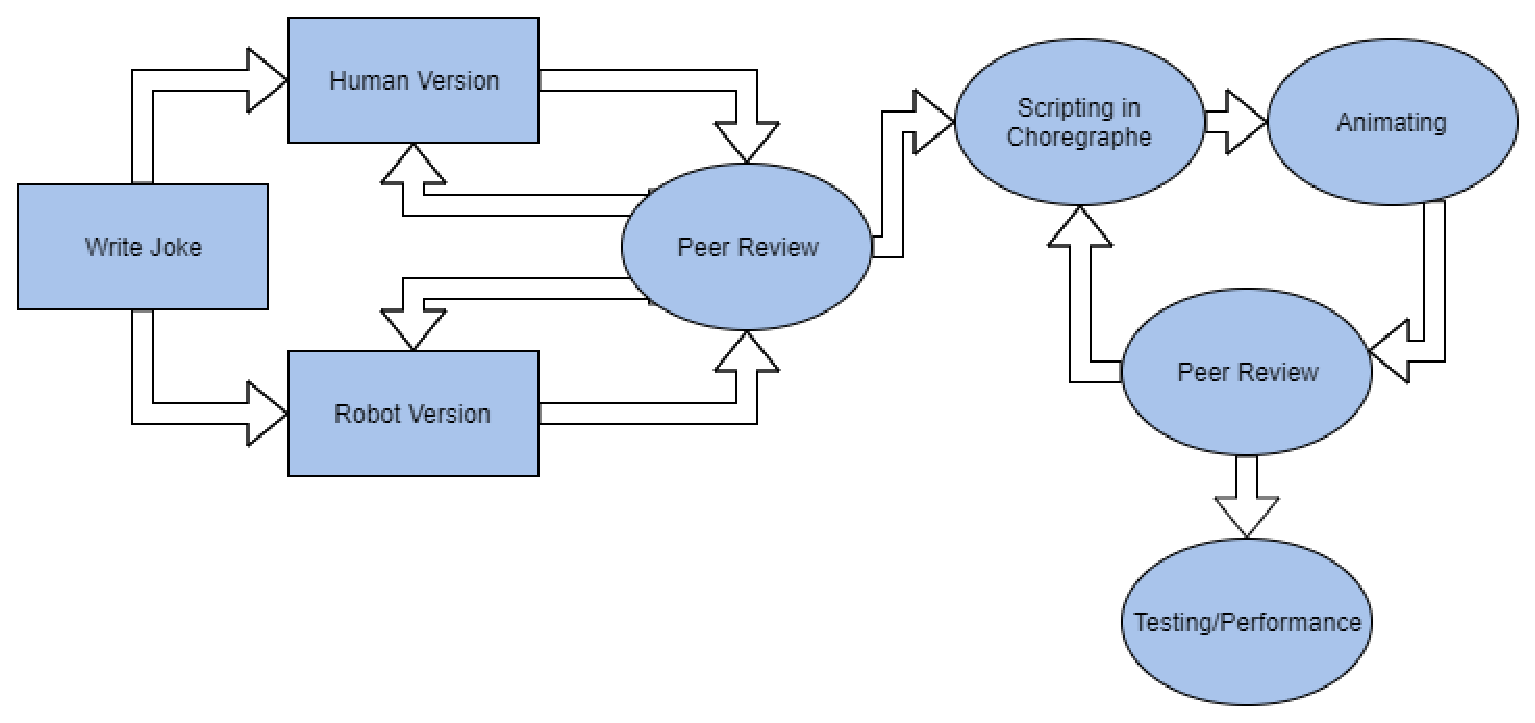
\includegraphics[width=0.75\textwidth,height=0.75\textheight,keepaspectratio]{joke_writing_process}
  \caption{The work flow from joke writing to testing.}
	\label{fig:write_process}
\end{figure}

\subsubsection{Experimentation}
The stand-up routine of the robot will comprise of text of the joke themselves, the motions that the robot uses to accompany them, and the way the robot surveys the audience after each punchline, e.g., in a human or robotic fashion.
To determine the differences in audience response to the routines, studies will be done first on Amazon Mechanical Turk, and later with co-located audiences.
Participants will be shown a video of the robot's stand-up routine, and then presented with a short survey.
The routines will be between 5 and 10 minutes long, and the survey will include questions pertaining to each joke or routine.
Participants will be compensated with standard rates for watching brief videos and answering survey questions.


\section{Conclusion}

Our project is coming together slowly, but surely. There are a lot of aspects we have accomplished successfully. It is just the matter of putting everything together and structuring the performances to make each one feel coherent and authentic.

\pagebreak


% \bibliographystyle{IEEEtran}
% \bibliography{refs}

\end{document}
